\documentclass[a4paper,oneside,DIV=12,12pt]{scrartcl}

\usepackage{graphicx}

%%% Load fonts
\usepackage{fontspec}
\setromanfont[
	SmallCapsFeatures = {LetterSpace = 5}
]{STIX Two Text}
\setsansfont{Roboto}
\setmonofont{PT Mono}

\usepackage{amsmath,unicode-math}
\setmathfont{STIX Two Math}
%%%

%%% Language-specific setup
\usepackage{polyglossia}
\setmainlanguage{ukrainian}
%%%

%%% Microtypographic enhancements
\usepackage{microtype}
%%%

%%% Table typesetting
\usepackage{booktabs}
%%%

%%% Math typesetting
%%%

%%% Problem-solution typesetting
\usepackage{xsim}
\loadxsimstyle{runin}
\DeclareExerciseTranslations{exercise}{
	Ukrainian	=	завдання ,
}

\DeclareExerciseTranslations{solution}{
	Ukrainian	=	розв'язання ,
}

\xsimsetup{
	solution/print = true,
	exercise/template = runin,
	solution/template = runin,
}
%%%


%%% Schematic elements typesetting
\newcommand{\schel}[1]{\textit{#1}}
%%%

%%%
\newcommand{\sheetno}[1]{{\centering\scshape\bfseries Білет~№{#1}\par}}
%%%

\begin{document}
	\begin{titlepage}
		\begin{center}
			Міністерство освіти і науки України\\
			Національний авіаційний університет\\
			Навчально-науковий інститут комп'ютерних інформаційних технологій\\
			Кафедра комп'ютеризованих систем управління
			
			\vspace{\fill}
				Академічна різниця\\
				з дисципліни:\\
				«Комп'ютерна логіка»\\
				II~семестр
				
			\vspace{\fill}
			
			\begin{flushright}
				Виконав:\\
				студент ННІКІТ СП-225\\
				Клокун Владислав\\
			\end{flushright}
			Київ~2017
		\end{center}
	\end{titlepage}
	
	\sheetno{16}
	
	\begin{exercise}
		Описати множення чисел, поданих паралельним кодом третім способом. Принцип множення. Навести операційну схему пристрою для виконання операцій множення чисел третім способом та надати пояснення її функціонування.
		
		Розрядність операндів: знак числа~— 1~розряд; число~— 10~розрядів.
	\end{exercise}
	
	\begin{solution}
		Під час множення чисел у прямих кодах знакові та основні розряди оброблюються окремо. Для визначення знака добутку здійснюють додавання по модулю~2 тих цифр, що розміщуються в знакових розрядах співмножників.
		
		Нехай множники~$Y$ та $X$~— правильні двійкові дроби вигляду $X = 0, x_1, x_2, \dots, x_n$, $Y = 0, y_1, y_2, \dots, y_n$, де $x_i, y_i \in \left\{0, 1\right\}$. Тоді добуток~$Z$ абсолютних величин чисел~$Y$ та~$X$ дорівнює:
		\begin{equation}
		\label{eqn:multiplication-general-form}
			Z = YX
			  = Y \cdot x_1 \cdot 2^{-1}
			  + Y \cdot x_1 \cdot 2^{-2}
			  + \ldots
			  + Y \cdot x_i \cdot 2^{-i}
			  + \ldots
			  + Y \cdot x_n \cdot 2^{-n}.
		\end{equation}
		
		Множення двох чисел $X$ та~$Y$ може бути реалізоване шляхом виконання визначеного циклічного процесу, характер якого залежить від конкретної форми виразу. Один цикл множення складається з додавання чергового часткового добутку, який є добутком множника~$X$ на одну цифру множника~$Y$, до суми часткових добутків.
		
		Для реалізації третього способу множення подамо вираз~\eqref{eqn:multiplication-general-form} у такому вигляді:
		\[
			Z =
			\left(
				\left(
					\left(
						0
						+ Y \cdot 2^{-1} \cdot x_1
					\right)
					+ Y \cdot 2^{-2} \cdot x_2
				\right)
				+ \ldots
				+ Y \cdot 2^{-i} \cdot x_i
			\right)
			+ \ldots
			+ Y \cdot 2^{-n} \cdot x_n.
		\]
		
		Суму часткових добутків у~$i$-му циклі ($i \in \left\{ 1, \dots, n \right\}$) можна одержати за формулою
		\[
			Z_i = 2 Z_{i - 1} + Y 2^{-n} x_i,
		\]
		де початкові значення $i = 1$, $Z_0 = 0$.
		
		При використанні такого способу множення здійснюється зі старших розрядів множника~$X$, сума часткових добутків зсувається вліво, а множник~Y нерухомий.
		
		\begin{figure}[!htbp]
		\centering
			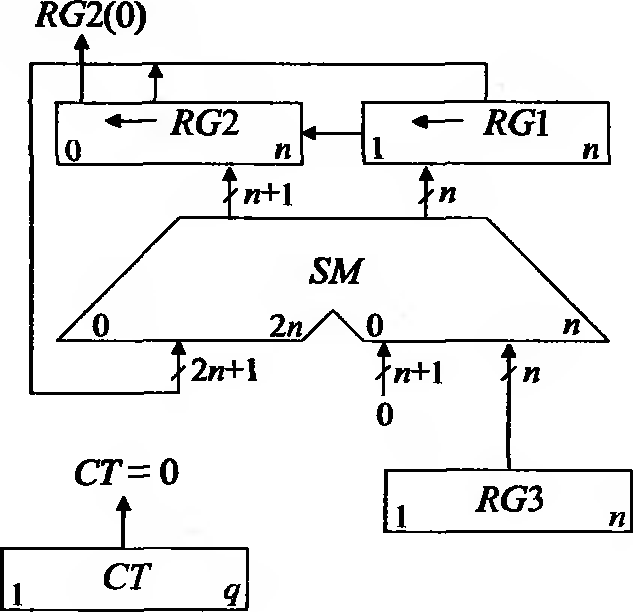
\includegraphics[height = 10\baselineskip]{assets/01-multiplication-3rd-method-operation-scheme.png}
		\caption{Операційна схема пристрою для множення чисел третім способом}
		\label{fig:multiplication-3rd-method-operation-scheme}
		\end{figure}
		
		Перед початком множення регістр~\schel{RG1} встановлюється в нульовий стан. Лічильник~\schel{CT} забезпечує підрахунок кількості циклів, тому при виборі розрядність лічильника необхідно це враховувати.
		
		Під час множення третім способом (операційна схема пристрою наведена на~рис.~\ref{fig:multiplication-3rd-method-operation-scheme}) вага молодшого розряду \schel{RG3} дорівнює $2^{-2n}$, тому код у регістрі \schel{RG3} є значенням $Y \cdot 2^{-n}$. На початку кожного циклу множення здійснюється лівий зсув у регістрах \schel{RG1} і~\schel{RG2}, а потім виконується додавання, яким керує \schel{RG2(1)}. У результаті додавання вмісту \schel{RG3} і~\schel{RG1} може виникнути перенос у молодший розряд регістру \schel{RG2}. У старшій частині суматора, на якому здійснюється додавання коду \schel{RG2} з нулями, відбувається поширення переносу. Збільшення довжини \schel{RG2} на один розряд усуває можливість поширення переносу в розряди множника. Після виконання $n$ циклів молодші розряди добутку будуть знаходитись в регістрі \schel{RG1}, а старші~— в регістрі \schel{RG2}. Час множення третім способом визначається за формулою $t_{\text{і}} = n \left( t_{\text{ї}} + t_{\text{с}} \right)$.
	\end{solution}
	
	\begin{exercise}
		Виконати операцію додавання чисел $A$ і~$B$ у форматі з плаваючою комою згідно чотирьох етапів. Виконати дію округлення результату. Додавання виконувати у модифікованому доповнювальному коді.
		
		У процесі додавання кількість розрядів мантис чисел $A$ і $B$ може бути збільшена до необхідних значень, але результат додавання після округлення повинен бути в~межах наданої розрядної сітки: $n$~розрядів для порядку і $m$~розрядів для мантис чисел~$A$ і~$B$ (без урахування кількості розрядів~знака).
		\[
			A = -\frac{37}{16}, \quad
			B = \frac{259}{128}, \quad
			n = 6, \quad
			m = 8.
		\]
		
		Результат множення чисел $A$ і $B$ надати у прямому коді. 
	\end{exercise}
	
	\begin{exercise}
		Побудувати функціональну схему пристрою з розподіленою логікою для обчислювальної функції~$D$.
		\[
			D = (-1 / 4) \cdot C - 8A \cdot (B - 1).
		\]
		Надати пояснення та обгрунтування функціонування пристрою. Кількість розрядів для кожного з операндів $A$, $B$, $C$ дорівнює $n$ без урахування розрядів знака. Операцію множення виконувати четвертим способом.
	\end{exercise}
\end{document}